%%==================================================
%% chapter4.tex for BIT Master Thesis
%% version: 0.1
%% last update: Nov 8th, 2017
%%==================================================
\chapter{离散时间半参数自适应控制}\label{chap:4}
自适应控制中的辨识是为了控制问题,上一章设计了二维情形下的信息浓缩估计算法去辨识线性部分的未知参数。本章将在第三章的基础上设计非参数部分的估计算法,主要借助于一种机器学习算法,然后根据两部分不确定性的估计结果设计自适应控制律,解决随动控制问题。

\section{问题描述}\label{sect:4.1}
再次考虑第二章给出的半参数模型
\begin{equation}%
\label{eq:4.semi-u}
y_{k+1} = \bm{\theta}^{\tau}\bm{\phi_{k}}+u_{k}+f(\bm{\bm{\psi}_{k}})+\epsilon_{k+1}
\end{equation}
其中,$\bm{\theta}$是未知参数向量,$f(\cdot)$是未知函数。同理,令
\begin{equation}
z_{k} = f(\bm{\psi}_{k}) + \epsilon_{k+1}
\end{equation}

针对系统\eqref{eq:4.semi-u},自适应估计与控制问题的一般表述是:给定关于$\bm{\theta}$,$f(\cdot)$和$\epsilon_{k+1}$的先验信息,在$k$时刻,如何根据实时产生的一系列输入输出数据$\{y_{k},u_{k};k=1,2,\ldots\}$,去估计未知参数$\bm{\theta}$和$z_{k}$?然后根据$\bm{\theta}$和$z_{k}$的估计(预测)值去设计合适的自适应控制输入$u_{k}$使得$k+1$时刻的输出$y_{k+1}$能跟踪上期望的输出$y_{k+1}^{*}$。

本章针对系统\eqref{eq:4.semi-u}有如下先验信息:
\begin{itemize}
\item 期望跟踪信号$\{y_{k}^{*}\}$是有界的,即存在有界正常数$B_{yd}$,使得
\begin{equation}\label{eq:4.ydB}
|y_{k}^{*}|\leq B_{yd},\ \forall k\geq0.
\end{equation}
\item $\bm{\theta}$各分量是有界的,即$\underline{\theta}_{j}\leq\theta_{j}\leq\overline{\theta}_{j}$,其中$\underline{\theta}_{j}$和$\overline{\theta}_{j}$为已知的常数,$j=1,2,\ldots,d_{1}$.
\item 噪声序列$\epsilon_{k}$的取值在一个已知的范围内,即
\begin{equation}\label{eq:4.wB}
\underline{\epsilon}\leq\epsilon_{k}\leq\overline{\epsilon},\ \forall k\geq0.
\end{equation}
\item 未知函数$f(\cdot)$的上下界受限于其他已知函数,即
\begin{equation}\label{eq:4.fB}
\underline{f}(\bm{\psi})\leq f(\bm{\psi})\leq \overline{f}(\bm{\psi}).
\end{equation}
\end{itemize}

第三章已经给出了$\bm{\theta}$的估计算法,因此剩下的部分可以分为两个核心问题,一方面是设计$f(\cdot)$的估计算法,另一方面是设计控制输入$u_{k}$的表达式。假设第二章设计出的未知参数的估计值为$\hat{\bm{\theta}}_{k}$,下面需要设计出$\breve{z}_{k}$的表达式。因此,根据必然等价原理,设计出的控制输入的一般表达式为:
\begin{equation}\label{eq:4.uk}
u_{k}^{*}=y_{k+1}^{*}-\bm{\phi_{k}}^{\tau}\cdot\hat{\bm{\theta}}_{k}-\breve{z}_{k}
\end{equation}
非线性部分的辨识与控制器的设计是本章要重点解决的问题。

\section{非参数部分的估计}\label{sect:4.2}
\subsection{最近邻估计}
前面的章节用信息浓缩估计解决了参数不确定性的辨识问题,现有的半参数自适应控制方法针对非参数部分使用的是最近邻估计,其针对的主要是一维参数情形($d_{1}=1$且$d_{2}=1$),即下面的一维半参数系统
\begin{equation}%
\label{eq:4.1ord}
y_{k+1}=\theta y_{k}+u_{k}+f(y_{k})+\epsilon_{k+1}
\end{equation}
这里,标量$\theta$是未知的,为系统的参数不确定性部分,同样$f(\cdot)$是非参数不确定性部分,满足Lipschitz条件。最近邻估计不显式地估计$f(\cdot)$部分,而是直接估计
\begin{equation}\label{eq:4.nne.g}
\eta_{k} = \theta y_{k}+f(y_{k})
\end{equation}
这个整体。这样,在用信息浓缩算法估计出参数$\theta$之后,移除这个估计值$\hat{\theta}$,就可以获得非参数部分的估计。

在系统\eqref{eq:4.1ord}中,由于Lipschitz条件的存在,不管是非参数部分还是参数部分都主要和输出值$y_{k}$相关,这样输出值$y_{k}$相近的时刻,那么$\eta_{k}$的值也应该相差不大。因此最近邻估计就主要利用到了这一点,其主要思想在于寻找和当前时刻输出值$y_{k}$最相近的时刻,然后进行比较计算。

首先定义最近邻时刻为
\begin{equation}\label{eq:4.it}
i_k\triangleq\mathop{\arg \min}\limits_{i<k}|y_k-y_i|
\end{equation}
$i_k$是历史输出值中和当前时刻最接近的时刻。那么有如下等式成立
\begin{equation*}
\begin{array}{lll}
&\eta_k&=\eta_k-z_{i_k}+z_{i_k}\\
&&=[\theta y_k+f(y_k)]-[\theta y_{i_k}+f(y_{i_k})+w_{i_k+1}]+z_{i_k}\\
&&=[\theta(y_k-y_{i_k})+z_{i_k}]+[f(y_k)-f(y_{i_k})-w_{i_k+1}]
\end{array}
\end{equation*}
一般来说,上面等式中的最后一行中$f(y_k)-f(y_{i_k})$的值接近零,并且干扰项比较小。因此,可以取整体表达式\eqref{eq:4.nne.g}的估计为
\begin{equation}\label{eq.4:g.est}
\begin{array}{lll}
\hat{\eta}_k&\triangleq\hat{\theta}_k(y_t-y_{i_k})+z_{i_k}
&=\hat{\theta}_{k}(y_k-y_{i_k})+(y_{i_k+1}-u_{i_k})
\end{array}
\end{equation}

接着,令
\begin{equation}\label{eq.4:bk}
\begin{array}{lll}
\bar{b}_k\triangleq \max\limits_{i\leq k}y_i
         =\max(\bar{b}_{k-1}, y_k)\\
\underline{b}_k\triangleq \min\limits_{i\leq k}{y_i}
                =\min(\underline{b}_{k-1}, y_k).
\end{array} 
\end{equation}

最后基于设计出下面的控制律
\begin{equation}\label{eq:4.uk}
u_{k}=\left\{
\begin{array}{cc}
  -\hat \eta_k+y_{k+1}^* & \text{if } |y_k-y_{i_k}|\le D \\
  -\hat \eta_k+\frac12(\bar b_k+\underline b_k) & \text{if } |y_k-y_{i_k}|> D \\
\end{array}
\right.
\end{equation}
这里,$D$是一个合适的常数值。

由此看出,最近邻估计可以比较准确地给出一维情形下非参数部分的估计,从而解决半参数系统的自适应控制问题。但是有一定的局限性,主要体现在:
\begin{enumerate}
\item 由于最近邻时刻$i_k$的计算需要遍历所有的历史值,因此,随着时间的增长,理论上需要无限的内存用来存储历史数据。这给实施带来了困难。
\item 由于在计算$\hat{g}_k$时没有对干扰值作特别处理,因此适用于干扰值的有界范围比较小且变化比较慢的系统。
\item 没有充分利用历史数据和关联先验信息,只是利用最近邻时刻的数据,计算结果不一定是最优的。
\end{enumerate}

以上的缺点存在,导致现有的半参数自适应控制存在很大的局限性。本章借助于其他的非线性辨识算法去设计新的非参数部分的估计算法。

\subsection{神经网络}
机器学习解决的问题从数学上主要分为分类和回归。其中分类处理的数据主要是离散型数据,回归解决的对象和思路跟控制中的估计、预测十分类似。而神经网络作为一种十分有效的回归与预测算法,在非线性辨识中应用十分广泛。神经网络主要由输入层、隐含层和输出层组成(最简单的神经网络可能没有隐含层),依据不同的激活函数或者不同的学习算法,种类十分丰富。

本章以及本文主要讨论一种十分常见的单隐层前馈神经网络(Single hidden layer feedforwar network, SLFN),即具有一个输入层、一个隐含层以及一个输出层的前馈型神经网络。这是一种多层网络,其中输入层神经元接受外界输入,隐含层与输出层的神经元对信号进行加工,最终结果由输出层神经元输出。

下面首先阐述神经网络的基本数学模型。对于一个具有$N_{i}$个输入神经元、$N_{o}$个输出神经元以及$N_{h}$个隐含层神经元的单隐层前馈神经网络来说,如果其激活函数为$g(\cdot)$,并存在$N_{s}$个输入输出样本对
$$\{\bm{x}_{j},\bm{t}_{j}\},\ j=1,2,\ldots,N_{s}$$
这里,输入向量为
$$\bm{x}_{j}=[x_{j,1},x_{j,2},\ldots,x_{j,N_{i}}]^{\tau}\in \mathcal{R}^{N_{i}}$$
期望的输出向量为
$$\bm{t}_{j}=[t_{j,1},t_{j,2},\ldots,t_{j,N_{o}}]^{\tau}\in \mathcal{R}^{N_{o}}$$
则对于任意输入向量$\bm{x}_{j}$,第$l$个($l=1,2,\dots,N_{o}$)输出层神经元的输出为
\begin{equation}%
\label{eq:4.slfn.o}
\begin{split}%
o_{j,l}&=\sum_{i=1}^{N_{h}} \beta_{i,l} g(\bm{w}_{i},b_{i},\bm{x}_{j})\\
&=\sum_{i=1}^{N_{h}} \beta_{i,l} h(\bm{x}_{i})\\
&=\bm{h}(\bm{x}_{j})^{\tau}\cdot\bm{\beta}_{l}
\end{split}
\end{equation}
其中,$\bm{w}_{i}$和$b_{i}$分别是连接第$i$个隐层神经元与输入层的权重向量和阈值,$\bm{\beta}_{l}$是连接$l$个输出层神经元和隐含层的权重,$\bm{h}(\bm{x}_{j})$为隐含层的输出向量。

一般来说,同一层的激活函数是一致的。如果第$i$个隐含神经元的激活函数$g(\cdot)$是加性的(addictive),比如Sigmoid型或者正弦型,则其输出为
\begin{equation}%
g(\bm{w}_{i},b_{i},\bm{x}_{j})=g(\bm{w}_{i}^{\tau}\cdot\bm{x}_{j}+b_{i})
\end{equation}
如果是径向基(Radias base function, RBF)网络,则
\begin{equation}%
g(\bm{w}_{i},b_{i},\bm{x}_{j})=g(b_{i}\|\bm{x}_{j}-\bm{w}_{i}\|)
\end{equation}
此时,$g$是某种径向对称的标量函数,通常定义为关于样本到数据中心$\bm{w}_{i}$之间的欧氏距离的单调函数,比如高斯径向基函数等。这样,在命名上,$\bm{w}_{i}$和$b_{i}$一般不称为隐层的权重和阈值,而是激活函数的中心(center)和影响因子(impact factor)。

理论上,对于给定的样本数据集,上述定义的具有$N_{h}$个隐含层神经元和激活函数为$g(\cdot)$的SLFN,具有零误差逼近$N_{s}$个样本的性质,即
\begin{equation*}
\sum_{j=1}^{N_{h}}\|o_{j}-t_{j}\|=0,\ j=1,2,\dots,N_{s}
\end{equation*}
这意味着,存在一组$\bm{w}_{i}$、$b_{i}$和$\bm{\beta}$,使得
\begin{equation}
\bm{h}(\bm{x}_{j})\bm{\beta}=t_{j},\ j=1,2,\dots,N_{s}
\end{equation}
将上面$N_{s}$个方程堆积起来,写成紧凑的矩阵形式就是
\begin{equation}\label{eq:4.nn.HT}
\bm{H}\bm{\beta}=\bm{T}
\end{equation}
其中,$\bm{H}$是隐含层的输出矩阵,具体为
\begin{equation}\label{eq:4.nn.H}
\begin{split}
&\bm{H}(\bm{w}_{1},\dots,\bm{w}_{N_{h}};b_{1},\dots,b_{N_{h}};\bm{x}_{1},\dots,\bm{x}_{N_{s}})=\\
&\begin{bmatrix}
&h(\bm{w}_{1},b_{1},\bm{x}_{1}) &\cdots &h(\bm{w}_{N_{b}},b_{N_{h}},\bm{x}_{N_{1}})\\
&\vdots &\cdots & \vdots\\
&h(\bm{w}_{1},b_{1},\bm{x}_{N_{s}}) &\cdots &h(\bm{w}_{N_{b}},b_{N_{h}},\bm{x}_{N_{s}})
\end{bmatrix}_{N_{s}\times N_{h}}
\end{split}
\end{equation}
\begin{equation}\label{eq:4.nn.beta}
\bm{\beta} = \begin{bmatrix}%
&\bm{\beta}_{1}^{\tau}\\
&\vdots\\
&\bm{\beta}_{N_{h}}^{\tau}
\end{bmatrix}_{N_{h}\times N_{o}}
\end{equation}
且
\begin{equation}\label{eq:4.nn.T}
\bm{T} = \begin{bmatrix}%
&\bm{t}_{1}^{\tau}\\
&\vdots\\
&\bm{t}_{N_{h}}^{\tau}
\end{bmatrix}_{N_{s}\times N_{o}}
\end{equation}

如果隐含层神经元个数等于样本的个数,即$N_{s}=N_{h}$,那么矩阵$\bm{H}$是方阵且可逆的,则SLFN可以实现零误差逼近的结果。然而,在实际的大多数情况下,隐含层神经元个数远小于样本个数,即$N_{h}\ll N_{s}$。这样,$\bm{H}$不是一个方阵,就不存在准确的一组$\bm{w}_{i}$、$b_{i}$和$\bm{\beta}$,使得$\bm{H}\bm{\beta}=\bm{T}$精确成立。这种情况下,神经网络学习的目标就是寻找合适的一组$\hat{\bm{w}}_{i}$、$\hat{b}_{i}$和$\hat{\beta}$,使得
\begin{equation}\label{eq:4.nn.H-T}
\begin{split}%
&\|\bm{H}(\hat{\bm{w}}_{1},\dots,\hat{\bm{w}}_{N_{h}};\hat{b}_{1},\dots,\hat{b}_{N_{h}})\hat{\bm{\beta}}-\bm{T}\|=\\
&\min_{\hat{\bm{w}}_{i},\hat{b}_{i},\hat{\bm{\beta}}}\|\bm{H}(\bm{w}_{1},\dots,\bm{w}_{N_{h}};b_{1},\dots,b_{N_{h}})-\bm{T}\|
\end{split}
\end{equation}
成立,等价于最小化下面这个基于累计误差的损失函数
\begin{equation}\label{eq:4.nn.cost}
E=\sum_{j=1}^{N_{s}}(\bm{h}(x_{j})\bm{\beta}-\bm{t}_{j})^{2}.
\end{equation}

多层网络的学习能力依赖于强大的学习算法,误差反向传播(error BackPropagation, BP)是一种十分经典的代表。迄今为止,现实中的神经网络都是使用BP算法进行训练,不仅仅局限于多层前馈神经网络,还适用于递归神经网络等其它类型。BP算法是一种基于梯度下降(gradient-descent-based)的学习算法。将需要调整的权重$\bm{w}_{j}$和$\bm{\beta}$以及阈值$b_{j}$等网络参数,整体记作向量$\bm{W}$,则BP算法按照下面的式子调整$\bm{W}$:
\begin{equation}\label{eq:4.bp.W}
\bm{W}_{k} = \bm{W}_{k-1}-\eta\frac{\partial E(\bm{W})}{\bm{W}},
\end{equation}
其中,$\eta$是学习速率。

\begin{algo}
\caption{$\mathbf{BP}$学习算法的主要流程}
\label{alg.bp}
\begin{algorithmic}%
\REQUIRE 训练样本集$\{\bm{x}_{j},\bm{t}_{j}\},\ j=1,2,\ldots,N_{s}$;\\
学习速率$\eta$;\\
迭代次数上限$N_{max}$\\
\STATE 初始化所有网络参数(随机选择,或者根据经验指定)
\FOR{$m=1$ to $N_{max}$}
  \STATE 根据输入样本和当前参数计算所有样本的输出结果;
  \STATE 计算输出层的累计误差;
  \STATE 将误差逆向传递至隐层神经元,根据隐层神经元的误差来对连接权重和阈值进行调整;
  \STATE 根据方程\eqref{eq:4.bp.W}更新$\bm{W}$;
  \STATE 判断累积误差是否达到停止条件,如果达到,则退出当前循环;否则,继续当前迭代过程;
\ENDFOR
\ENSURE 网络参数向量$\bm{W}$确定的前馈型神经网络\\
\end{algorithmic}
\end{algo}

在前馈型神经网络中,BP算法的主要工作流程见算法\eqref{alg.bp}。从学习过程可以看出,BP算法存在如下问题:
\begin{enumerate}
\item 学习速率$\eta$的大小会影响算法的迭代过程,主要表现在,如果$\eta$太大,则算法会变得不稳定且可能会发散;如果$\eta$太小,则收敛速度非常慢。
\item 本质上是基于梯度的搜索寻优方法,会陷入局部最优的困境,即网络参数的更新会收敛到某个误差局部最小的情况,这是梯度下降所导致的。
\item 神经网络可能存在过度训练、过度拟合的情形,以致于网络的泛化能力很差。
\item 从初始解出发,迭代寻找最优参数值,其过程通常非常耗时,难以做到实时在线计算。
\end{enumerate}

以上这些因素对于神经网络在控制系统中的应用带来了很多问题,前面三条包括学习速率、局部最优、过度训练的问题有一些方法去改进,但是第四条迭代过程耗时这个问题是由梯度算法本身的特性所决定,难以从根本上解决。这就导致了超限学习机的提出。

\subsection{ELM及其变体}
传统上对于神经网络的理解,都认为需要网络的学习过程需要调整所有的参数。但实际上,如果输入层到隐含层的权重和阈值不变,那么隐含层的输出矩阵$\bm{H}$就保持不变,仅调整隐含层到输出层的权值就可以改变整个网络的最终输出。超限学习机就是利用这个思路建立起来的,用来解决传统基于梯度学习算法的耗时训练的缺点。

超限学习机的基本算法主要包括三个步骤,针对单隐层前馈神经网络的学习过程见算法\ref{alg.elm}。
\begin{algo}
\caption{$\mathbf{ELM}$算法}
\label{alg.elm}
\begin{algorithmic}%
\REQUIRE 训练样本集$\{\bm{x}_{j},\bm{t}_{j}\},\ j=1,2,\ldots,N_{s}$\\
\STATE Step1: 随机初始化输入权重$\bm{w}_{i}$和阈值$b_{i}$参数
\STATE Step2: 计算隐含层输出矩阵$\bm{H}$,见表达式\eqref{eq:4.nn.H}
\STATE Step3: 计算输出层权重向量$\bm{\beta}$,根据如下表达式
\begin{equation}\label{eq:4.elm.beta}
\bm{\beta}=\bm{H}^{\dag}\bm{T}
\end{equation}
其中$\bm{H}$、$\bm{T}$和$\bm{\beta}$的定义分别见方程\eqref{eq:4.nn.H}、\eqref{eq:4.nn.T}和\eqref{eq:4.nn.beta},而$\bm{H}^{\dag}$代表了矩阵$\bm{H}$的Moore-Penrose广义逆。
\ENSURE 网络参数向量$\bm{W}$确定的前馈型神经网络\\
\end{algorithmic}
\end{algo}

图\eqref{fig:elm}表示的是ELM在单隐层神经网络学习过程中的主要计算步骤。实际上,\eqref{eq:4.elm.beta}计算的是方程\eqref{eq:4.nn.HT}的最小二乘解(通常也是最小范数解),即
\begin{equation}
\bm{\beta}=(\bm{H}^{\tau}\bm{H})^{-1}\bm{H}^{\tau}\bm{T} 
\end{equation}

\begin{figure}
 \centering
 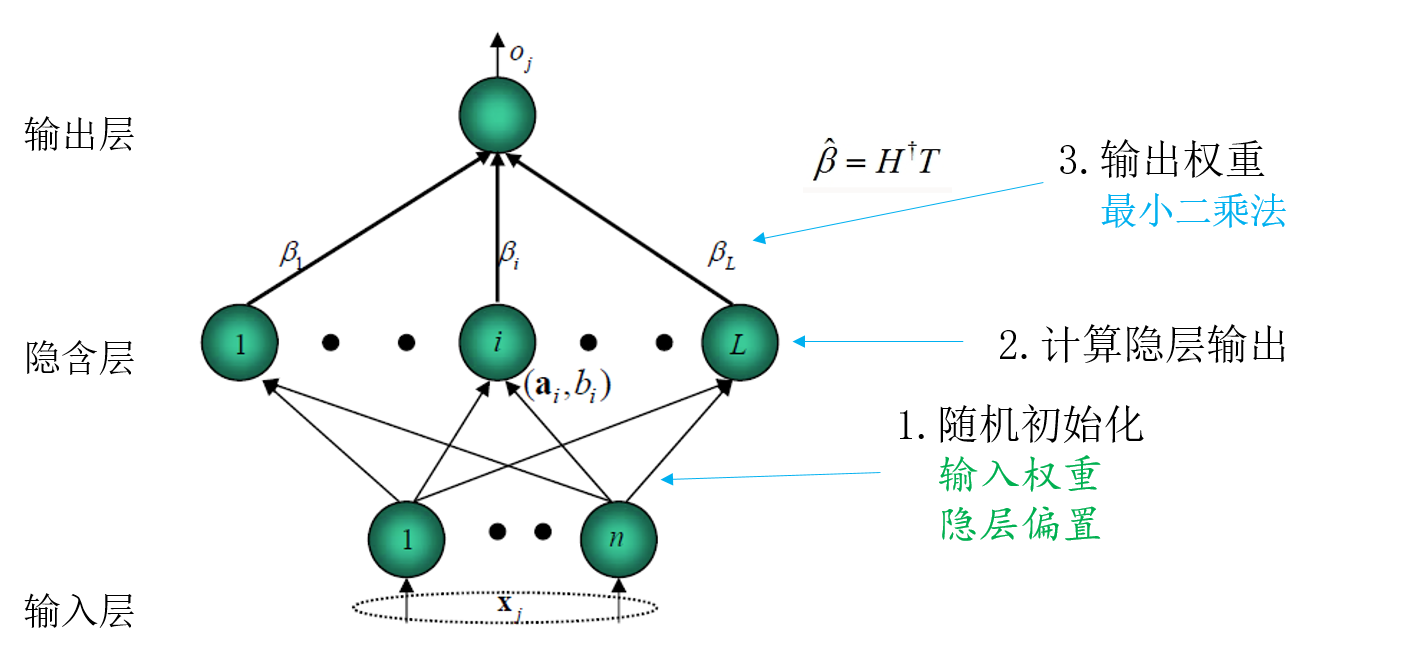
\includegraphics[width=0.7\textwidth]{ch1-ELM.png}
 \caption{超限学习机的网络结构(单隐层前馈型)和算法流程}\label{fig:elm}
\end{figure}

由于没有迭代过程,因此ELM在解决分类或者回归等问题时学习时间很短,主要耗时在矩阵的加减乘除和求逆运算的时间。从学习过程可以看出,ELM的求解思路和最优化方法以及最小二乘辨识算法有些相似,因此基本算法存在的问题和改进思路也类似。上述算法\ref{alg.elm}介绍的是原始ELM的批处理形式,由于实际中样本可能不是一次性获得的,因此和最小二乘算法一样,得到ELM的递推形式,即在线序列ELM算法(OS-ELM)\upcite{LiangHuang2006}。

OS-ELM的推导过程不再详细介绍,和RLS类似。OS-ELM对于控制系统的辨识十分有用,因为控制系统的数据大多是实时产生的,需要在线辨识。然而OS-ELM和批处理形式最后的效果是一致的,只是中间过程不一样,并没有对网络结构和目标函数进行优化。基本ELM优化的仅仅是经验损失风险,目标函数见\eqref{eq:4.nn.cost},因此ELM和OS-ELM都可能存在泛化能力不足和过拟合的现象。为了解决这个问题,相关学者\upcite{Escandell2011,HuynhWon2011}提出了正则化ELM(简称Re-ELM)和正则化OS-ELM(简称ReOS-ELM)。

神经网络在人工智能领域一直发挥重大作用,而人工智能的发展也一直推动着神经网络的研究。为了更好地利用神经网络实现预测和分类,特别是2012年之后,深度学习(Deep Learning, DL),借助于大量数据的驱动,在图像分类、语音识别、自然语言处理等应用领域中获得了巨大成功\upcite{ZhengChenZhang2014}。目前大部分深度学习算法大部分是基于神经网络建立。对于深度学习来说,隐含层的数量级为十几层到几百层不等,甚至上千层。深层网络结构和特征学习思想是深度学习的两大主要特点。针对大数据的应用,超限学习机也有相关变体,如H-ELM(
High-Performance Extreme Learning Machine)\upcite{AkusokBjork2015}与深度学习相比。超限学习机在不丢失精度的条件下具有快速的优势,比较见表\ref{tab:elm-dl}所示。可以看出,超限学习机不管是在在一般量级的数据样本和大数据学习应用领域都具有很大的潜力。
\begin{table}
\centering
\caption{超限学习机与常见深度学习算法的性能比较}\label{tab:elm-dl}
\begin{tabular*}{0.9\textwidth}{@{\extracolsep{\fill}}cccc}
\toprule
算法名称	&测试精度($\%$)	&训练时间 \\
\midrule
H-ELM	&99.14	&281.37s\\
Multi-layer ELM	&$99.03\pm0.04$	&281.37s\\
Deep Belief Networks(DBN)	&98.87	&20580s(5.7 hours)\\
Deep Boltzmann Machine(DBM)	&99.05	&68246s(19 hours)\\
Stacked Auto Encoders(SAE)	&98.6	&>17 hours\\
Stacked Denoising AutoEncodes(SDAE)	&98.72	&>17 hours\\
\bottomrule
\end{tabular*}
\end{table}

\subsection{ELM估计}
基于机器学习的辨识与建模是数据驱动的,可以适用于线性和非线性系统,主要建立系统的输入输出模型。快速、高精度的特点使得ELM迅速称为系统与控制领域很好的建模、估计与预测算法\upcite{LiJiaLiu2014}。特别是经过优化、提高泛化等方面性能的ELM变体算法,如Re-OSELM。不同于\eqref{eq:4.nn.cost}和\eqref{eq:4.nn.H-T},ReOS-ELM最小化目标的损失函数是
\begin{equation}\label{eq:4.re.cost}
\|\bm{H}\bm{\beta}-\bm{T}\|^{2}+\lambda\|\bm{\beta}\|^{2}
\end{equation}
正则化因子$\lambda$的引入提高了网络的泛化能力。图\eqref{fig.reoselm}展示了用Re-OSELM建立非线性模型的框图。

\begin{figure}[!htb]
  \centering
  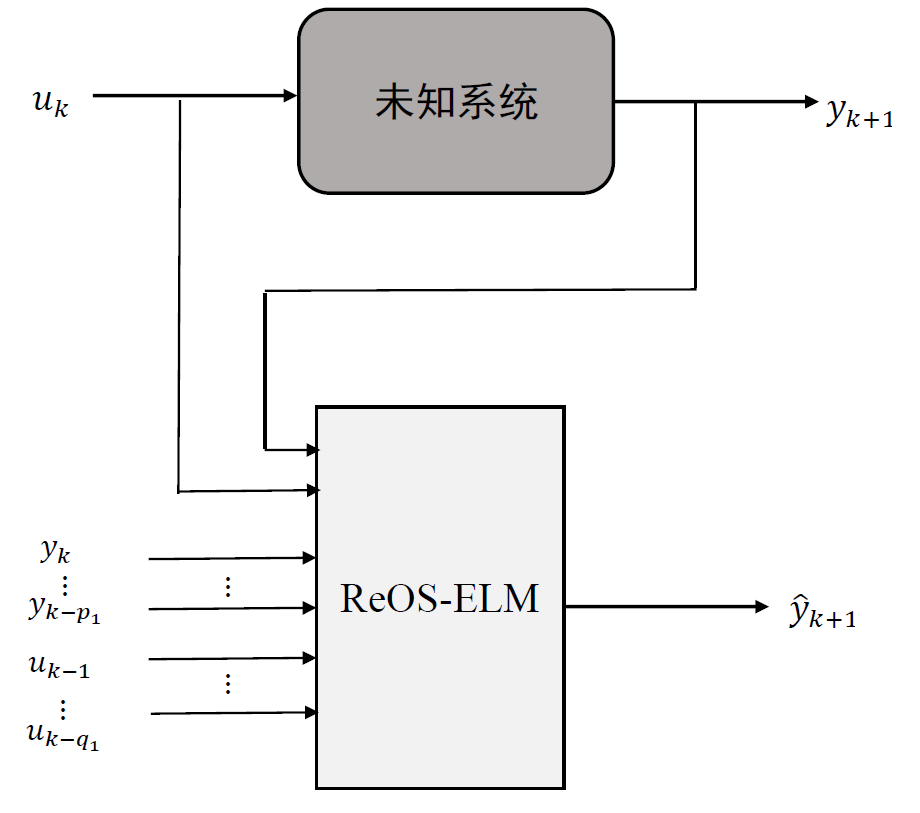
\includegraphics[width=0.6\textwidth ]{ch4-re-elm-c.png}\\	 % e.g.,[scale=0.75], [width=0.75\textwidth ]
  \caption{Re-OSELM算法的建模示意框图}
  \label{fig.reoselm}
\end{figure}

类似于RLS,OS-ELM和Re-OSELM等算法在系统建模与估计过程一般都是分为两个阶段。第一个阶段是初始化网络参数和输出权重$\bm{\beta}$估计值。对于Re-OSELM来说,需要一部分的离线输入输出数据用来完成初始化阶段,通过网络得出$\bm{H}_{0}$和$\bm{T}_{0}$之后,需要计算
\begin{equation}
\begin{split}%
\bm{P}_{0}&=(\bm{H}_{0}^{\tau}\bm{H}_{0}+\lambda \bm{I}_{N_{h}})^{-1}\\
\bm{\beta}^{0}&=\bm{P}_{0}\bm{H}_{0}\bm{T}_{0}
\end{split}
\end{equation}
这里,$\bm{I}_{N_{h}}$是$N_{h}\times N_{h}$的单位矩阵

在Re-OSELM算法更新权重的过称中引入恰当的或者自适应的遗忘因子$\rho$,可以使得算法能够应用到时变参数系统中。由于正则化因子$\lambda$的存在,即使不需要大于隐含层个数的样本数据用来初始化$\bm{\beta}^{0}$,初始小规模的训练集也是比不可少的。然而,在控制系统中,由于输出值跟实际输入密切相关,因此一定数量的离线输入输出数据一般情况下是难以获得的,这就限制了Re-OSELM在实际控制系统中的应用。

ITF-OELM算法就是用来解决缺少离线初始化数问题而提出的。ITF-OELM算法主要针对下面的单输入单输出离散时间非线性系统
\begin{equation}\label{eq:4.siso}
y_{k+1} = g(\bm{x}_{k})+\phi(\bm{x}_{k})u_{k}
\end{equation}
这里$\bm{x}_{k}$是由$\{u_{k},y_{k}\}$组成的回归向量,$g(\cdot)$和$\phi(\cdot)$是具有未知参数的未知非线性函数。用ITF-OELM算法分别估计$g(\cdot)$和$\phi(\cdot)$,得到$\hat{g}(\cdot)$和$\hat{\phi}(\cdot)$,那么基于ITF-OELM估计的自适应控制律为
\begin{equation}\label{eq:4.itf.u}
u_{k}=\frac{y_{k+1}^{*}-\hat{g}(\bm{x}_{k})}{\hat{\phi}(\bm{x}_{k})} 
\end{equation}
这里,$y_{k+1}^{*}$是期望的输出值。

基于ITF-OELM的自适应控制框图如图\ref{fig.itf-oelm}所示。ITF-OELM算法与Re-OSELM的不同点主要在于初始化输出权重的过程。前者不需要一定数量的离线数据,仅仅用第一组到达的数据初始化估计。另外,ITF-OELM还引入了再学习机制,即如果发现估计偏差较大,就重新初始化网络的所有参数,重新学习。这样,ITF-OELM可以应用于快时变系统,且不需要过多的离线数据。
\begin{figure}[!htb]
  \centering
  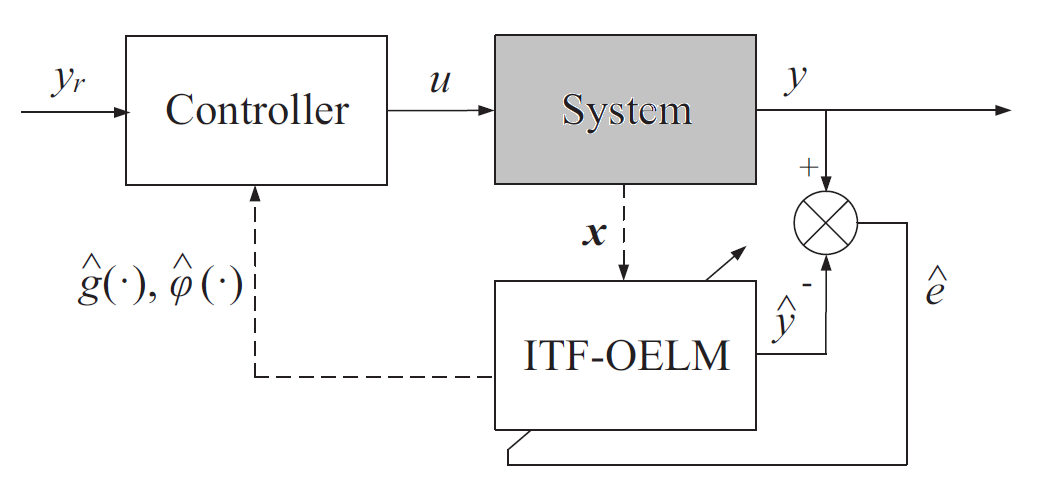
\includegraphics[width=0.7\textwidth ]{ch4-itf.png}\\	 % e.g.,[scale=0.75], [width=0.75\textwidth ]
  \caption{基于ITF-OELM的自适应控制框图}
  \label{fig.itf-oelm}
\end{figure}

下面借助ITF-OELM来解决本课题的非参数部分的估计问题。首先要确定的是网络的输入输出样本数据。本文要估计的非线性部分为
\begin{equation}
z_{k} = f(\bm{\psi}_{k}) + \epsilon_{k+1}
\end{equation}
因此,神经网络的输入是$d_{2}=p_{2}+q_{2}$维向量
$$\bm{\psi_{k}}=[y_{k},y_{k-1},\ldots,y_{k-p_{2}},u_{k-1},\dots,u_{k-q_{2}+1}]^{\tau}$$
$d_{2}$的具体数值视实际被控对象而定。输出是标量$z_{k}$。因此网络的输出层只有一个神经元,输入层含$d_{2}$个神经元。

本课题针对半参数系统在原始的ITF-OELM算法基础上做了几点变化。首先是估计的非线性函数只有一个,其次是在学习机制的不同。训练网络采用的输入数据$\bm{\psi}_{k}$直接来源于输入和观测到的历史输出数据,然而输出样本数据为
\begin{equation}\label{eq:4.hatz}
\hat{z}_{k-1}=y_{k}-\bm{\phi}_{k}^{\tau}\hat{\bm{\theta}}_{k-1}-u_{k-1}
\end{equation}
这个非线性估计部分是除去参数估计之后的剩余部分。用基于单隐层网络的ELM学习算法得到的估计值是
\begin{equation}\label{eq:4.z.breave}
\breve{z}_{k}=H_{k}\beta^{k}
\end{equation}

和其他监督学习算法一样,网络的训练结果依赖于样本数据的准确性。$\hat{z}_{k-1}$的值依赖于参数估计值$\hat{\theta}$,因此当参数估计值趋于稳定或者参数集合收敛到一定范围之后,需要重新初始化网络参数,继续辨识。也就是说,本课题在实施ITF-OELM算法时,不直接采用原本的再学习机制,而是引入另外一种情况下的再学习机制。这样就可以做到非参数估计更加准确。

本课题基于ELM算法估计非参数部分的实施过程依赖和控制密切相关,故具体算法公式将和自适应控制器设计一起在下一节介绍。

\section{自适应控制器}\label{sect:4.3}
\begin{figure}[!htb]
  \centering
  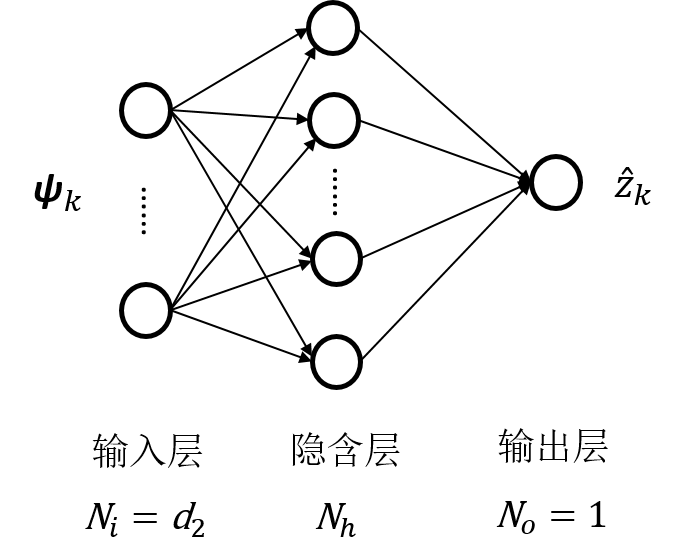
\includegraphics[width=0.55\textwidth]{ch4-elm-use.png}\\	 % e.g.,[scale=0.75], [width=0.75\textwidth ]
  \caption{半参数自适应控制系统中采用的单隐层前馈网络结构和参数}
  \label{fig.elm.use}
\end{figure}

\subsection{算法设计}\label{sect:4.3.1}
用信息浓缩估计参数部分,用ELM估计非参数部分,如图\ref{fig.elm.use}。在前面两种算法的基础上,可以设计出半参数自适应控制器\upcite{ZhouMaLiYang2017},主要包含两个过程,即初始化阶段和自适应控制阶段。在初始化阶段,需要完成信息浓缩估计器关联先验信息设置相关参数集的任务,以及ELM学习算法的网络参数初始化任务;自适应控制阶段前半段主要是参数估计,后半段主要是神经网络的学习更新非参数部分的估计,从而产生合适的控制输入,完成轨迹跟踪任务。

控制的目标是使得系统\ref{eq:4.semi-u}跟踪上期望的轨迹$y^{*}_{k},\ k\geq0$。下面介绍具体实施流程,其中信息浓缩估计部分直接针对二维参数情形设计。

\begin{enumerate}%
%1
\item \textbf{初始化阶段}
\begin{enumerate}%
%1.1
\item 设置$k=0$,系统的初始状态为
\begin{equation*}
\begin{split}%
\phi_{0}&=[y_{0},\ y_{-1}]^{\tau}\\
\psi_{0}&=[y_{0},\dots,,y_{-p_{2}},u_{-1},\dots,u_{-q_{2}+1}]
\end{split}
\end{equation*}
\item 根据关于$\bm{\theta}$的先验信息可以得到初始的多边形为$\Gamma_{0}$(通常是四边形),以及初始的参数估计$\hat{\bm{\theta}}_{0}$.
\item 定义SLFN网络的隐含层神经元个数$N_{h}$,正则化因子$\lambda$和遗忘因子$\rho$.
\item 对于第$i$个隐层神经元,随机初始化网络参数$(a_{i},b_{i})$,$i=1,2,\ldots,N_{h}$.
\item 设置$\beta^{0}$和$P_{0}$为
\begin{equation}\label{eq.elm0}
\begin{split}%
& P_{0} = (\lambda \bm{I_{N_{h}}})^{-1} \\
& \beta^{0} = \bm{0}_{N_{h}}
\end{split}
\end{equation}
这里,$\bm{I_{N_{h}}}$和$\bm{0}_{N_{h}}$分别记作$N_{h}\times N_{h}$的单位矩阵和$N_{h}\times1$的零向量。
\item 设置再学习机制参数。让$\sigma_{k}=var(C_{k})$代表在多边形区域$C_{k}$的所有顶点坐标的方差,即
\begin{equation}
\begin{split}%
\sigma_{n_{k}}(1) &= var(X_{P_{1}},X_{P_{2}},\ldots,X_{P_{n_{k}}}) \\
\sigma_{n_{k}}(2) &= var(Y_{P_{1}},Y_{P_{2}},\ldots,Y_{P_{n_{k}}})
\end{split}
\end{equation}
\item 设置$Flag=0$,意味着尚未激活再学习过程,并记$\delta$为学习方差的上限。
\item 随机产生一个有界的控制输入$u_{0}$,并发送给控制系统\eqref{eq:4.semi-u};设置$k=1$,然后转到Step 2(a).
\end{enumerate}
%2
\item \textbf{自适应控制阶段}
\begin{enumerate}%
%2.a
\item 获得系统在第$k$个时刻的输出值$y_{k}$,并利用第二章的公式\eqref{eq.fk}计算$v_{k,1}$和$v_{k,2}$.
%2.b
\item 用第三章的公式得到当前的多边形区域$C_{k}$,并将$C_{k}$的中心作为当前参数估计值$\hat{\bm{\theta}}_{k}$.
%2.c
\item 计算$\sigma_{k}$,如果$Flag=0\bigwedge\sigma_{k}(1)\leq\delta\bigwedge\sigma_{n_{k}}(2)\leq\delta$ 那么设置$\gamma=1$与$Flag=1$。
%2.d
\item 设置$\hat{z}_{k-1}=y_{k}-\phi_{k-1}^{\tau}\hat{\bm{\theta}}_{k}-u_{k-1}$.
%2.e
\item 如果$\gamma=1$那么执行(i); 否则,执行(ii).
\begin{enumerate}%
\item Updating:将$(\bm{\psi}_{k-1},\hat{z}_{k-1})$作为SLFN的输入输出样本数据,计算网络的隐含层输出$H_{k-1}$,并使用下面的等式计算矩阵$P_{k}$和隐含层到输出层的权重
\begin{equation}\label{eq.elmk}
\begin{split}%
P_{k}=&\frac{1}{\rho}(P_{k-1}-P_{k-1}H_{k-1}^{\tau}(\rho\\
&+H_{k-1}P_{k-1}H_{k-1}^{\tau})^{-1}H_{k-1}P_{k-1}) \\
\beta^{k}=&\beta^{k-1} + P_{k-1}H_{k-1}^{\tau}(\hat{z}_{k-1}-H_{k-1}\beta^{k-1})
\end{split}
\end{equation}
\item Relearning:执行在初始化阶段的步骤1-(c),1-(d),1-(e).
\end{enumerate}
\item 将$\bm{\psi}_{k}$作为SLFN的输入向量,并计算隐含层的输出矩阵$H_{k}$,从而得到非参数的估计
\begin{equation}\label{eq.hat.z.k}
\breve{z}_{k}=H_{k}\beta^{k}
\end{equation}
\item 结合参数和非参数两部分的估计,根据必然等价原理设计控制输入为
\begin{equation}\label{eq.4:u}
u_{k}=y^{*}_{k+1}-\phi_{k}^{\tau}\hat{\bm{\theta}}_{k}-\breve{z}_{k}
\end{equation}
\item 设置$k=k+1$,然后转到Step 2(a).
\end{enumerate}
\end{enumerate}

\subsection{稳定性分析}\label{sect:4.3.2}
下面针对系统\ref{eq:4.semi-u}和半参数自适应控制算法分析闭环特性。系统在$k+1$时刻的期望输出为$y^{*}_{k+1}$,实际输出值为$y_{k+1}$,则跟踪误差定义为
\begin{equation}
e_{k+1} = y_{k+1} - y^{*}_{k+1}.
\end{equation}
从方程\eqref{eq:4.semi-u}, \eqref{eq:4.hatz}和\eqref{eq.4:u},容易得到
\begin{equation}\label{eq:4.stab}
\begin{split}%
e_{k+1} & = y_{k+1} - y^{*}_{k+1}\\
& = y_{k+1} - \hat{y}_{k+1} + \hat{y}_{k+1} - y^{*}_{k+1}\\
& = (y_{k+1} - \phi_{k}^{\tau}\hat{\theta}_{k} - \breve{z}_{k} - u_{k} )+(\phi_{k}^{\tau}\hat{\theta}_{k} + \breve{z}_{k} + u_{k}  - y^{*}_{k+1})\\
& = \phi_{k}\theta_{k} + z_{k} - \phi_{k}^{\tau}\hat{\theta}_{k} - \breve{z}_{k}\\
& = \phi_{k}(\theta_{k} - \hat{\theta}_{k}) + (z_{k} - \breve{z}_{k})\\
& = \phi_{k}\tilde{\bm{\theta}}_{k}+\tilde{z}_{k}
\end{split}
\end{equation}
从上面的方程\eqref{eq:4.stab}可以看出,如果参数部分和非参数部分的估计误差$\tilde{\bm{\theta}}_{k}$和$\tilde{z}_{k}$收敛到零,那么跟踪误差$e_{k+1}$也收敛到零。前面一章设计的信息浓缩估计可以保证未知参数估计收敛到零,并且本章的ELM估计非参数部分也可以保证收敛性,因此,本章设计的半参数自适应控制器可以保证渐进稳定性。

\section{仿真实例}\label{sect:4.4}

\subsection{仿真环境}\label{sect:4.4.1}
本章验证自适应控制器的性能,选择仿真如下半参数被控对象
\begin{equation}\label{eq:4.plant}
y_{k+1} = \theta_{1}y_{k} + \theta_{2}y_{k-1} + u_{k} + f(y_{k},y_{k-1}) + \epsilon_{k+1} 
\end{equation}
其中,系统的未知参数和未知函数设定为
\begin{equation}
\begin{array}{c}
\theta_{1} = -1\textbf{, }\theta_{2} = 1\\
f(y_{k},y_{k-1}) = \sin(y_{k}^{2}) + \cos(y_{k-1})
\end{array}
\end{equation}
同时,未知的噪声序列是独立同分布(i.i.d)的随机有界均匀分布,取自$U(-0.1,0.1)$。该被控对象的参数部分是二维情形,非参数部分也是二维情形,即$p_{1}=2$同时$q_{2}=2$。系统可利用的先验信息在数学上描述为
\begin{equation}\label{eq.4:aprior}
\begin{split}
&\underline{f}(\psi_{k})=-3,\ \overline{f}(\psi_{k})=4\\
&\underline{\epsilon}=-0.1,\ \overline{\epsilon}=0.1\\
&\underline{\theta}_{1}=-10,\ \overline{\theta}_{1}=10\\
&\underline{\theta}_{2}=-10,\ \overline{\theta}_{2}=15
\end{split}
\end{equation}

为了更好的验证半参数自适应控制器的性能,本章选取了经典的自适应控制算法,即自校正控制器(STR)作为对比算法。自校正控制器(或者自校正调节器)采用最小二乘算法(RLS)估计未知参数。不过由于RLS针对的是线性系统,而本章要控制的对象是\eqref{eq:4.plant}是非线性的。对比仿真实验的唯一控制变量在于自适应控制算法,因此先验信息\eqref{eq.4:aprior}对于STR同样可以利用,需要对原生的RLS估计进行简单的改进,补偿掉非线性部分。

对比方法RLS实际估计的线性部分为
\begin{equation}\label{eq:4.zrls}
L_{k}\triangleq\theta_{1}y_{k} + \theta_{2} y_{k-1}=y_{k+1}-u_{k}-\hat{z}_{RLS}
\end{equation}
其中,$\hat{z}_{RLS}$是STR实施过程中对非线性部分的一个粗略估计,用来补偿掉非线性部分,具体值可取
\begin{equation}\label{eq:4.zhatrls}
\hat{z}_{RLS}=\frac12 (\underline{f}(\psi_{k})+\overline{f}(\psi_{k})) 
\end{equation}
RLS估计算法也包括两个过程,第一个是初始化过程确定初始值,即
\begin{equation}\label{eq:4.rls.0}
\begin{split}
&\bm{\pi}_{0}=\alpha \bm{I}_{d_{1}}\\
&\bm{\theta}^{0}=[0.1,\dots,0.1]^{\tau}
\end{split}
\end{equation}
$\alpha$取较大的数(一般为$10^{4}$到$10^{8}$之间)。第二阶段是递推过程,每一步都会改变$\bm{\theta}$和$\bm{\pi}^{0}$的值。第$k$时刻的估计为
\begin{equation}\label{eq:4.rls.k}
\begin{split}
\hat{\bm{\theta}}_{k}&=\hat{\bm{\theta}}_{k-1}+ \zeta_{k} \bm{\pi}_{k-1} \bm{\phi}_{k} (L_{k}-\bm{\phi}_k^\tau \bm{\theta}_{k-1})\\
\zeta_k&=(1+\bm{\phi}_{k}^{\tau} \bm{\pi}_{k-1} \bm{\phi}_{k})^{-1}\\
\bm{\pi}_{k}&=\bm{\pi}_{k-1}-\zeta_k \bm{\pi}_{k-1} \bm{\phi}_{k} \bm{\phi}_{k}^{\tau} \bm{\pi}_{k-1}
\end{split}
\end{equation}
方程\eqref{eq:4.zhatrls}到\eqref{eq:4.rls.k}就是本章对比仿真采用的RLS算法。

\subsection{仿真结果}\label{sect:4.4.2}
设定的期望跟踪信号为
\begin{equation}\label{eq:4.sim.yd}
y_{k}^{*} = 1.5\sin(2\bm{\pi} k\times T_{s})
\end{equation}
其中,控制周期为$T_{s}=0.01$s。仿真半参数自适应控制和自校正控制算法,得到系统的输出曲线分别为\ref{fig.sim.elm.sys}和\ref{fig.sim.str.sys}。在图\ref{fig.sim.elm.sys}中,可以看出半参数自适应控制的轨迹跟踪精度比较好,系统的实际输出很快的跟踪上了期望的输出,误差逐渐收敛到一个很小的范围。相反,自校正控制的跟踪效果就较差,经过一段时间后,系统的实际输出和期望值偏差仍然较大,如图\ref{fig.sim.str.sys}所示。在本节的仿真实例中,自适应控制的输出跟踪误差在自校正控制的基础上减少了大约10倍。
\begin{figure}[!htb]
	\centering
	\subfigure[输出轨迹]{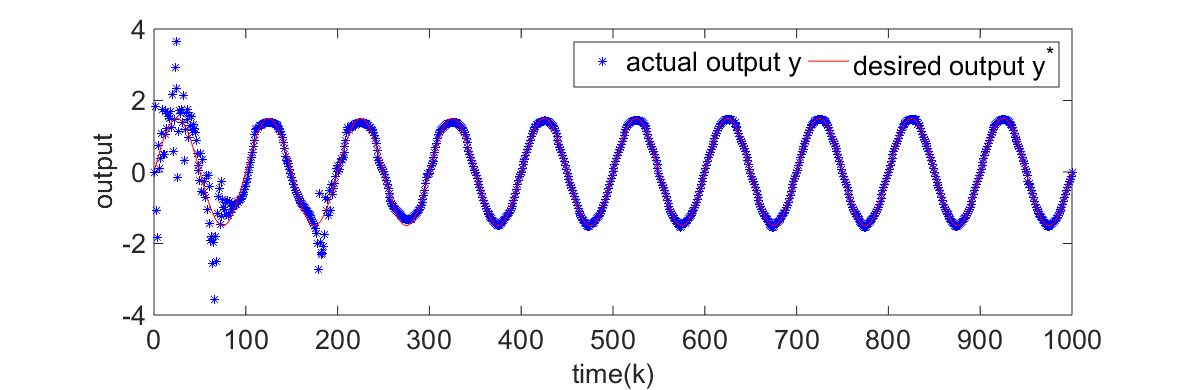
\includegraphics[width=0.65\textwidth ]{ch4-sim-elm-y.png}\label{fig.sim.elm.y}}\\
	\subfigure[跟踪误差]{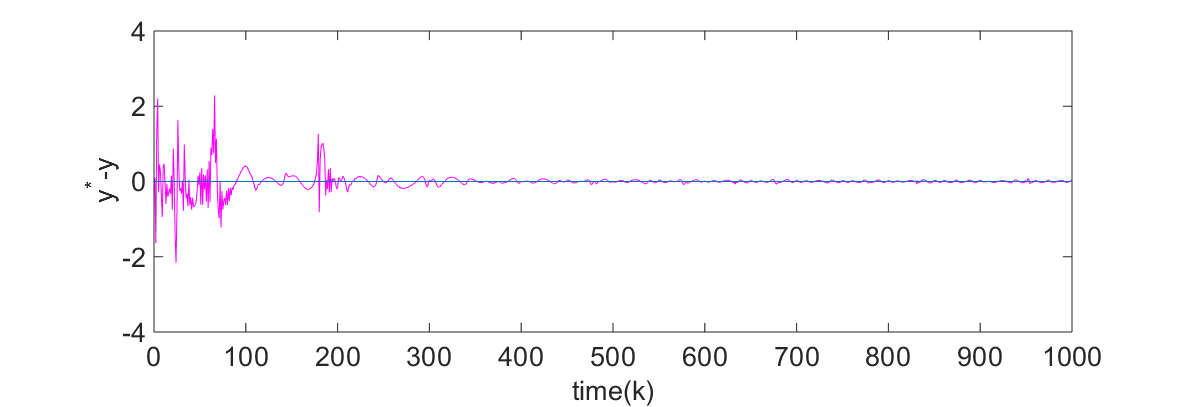
\includegraphics[width=0.65\textwidth ]{ch4-sim-elm-yerror.png}\label{fig.sim.elm.ye}}
	%\subfigure[控制输入]{\includegraphics[width=0.5\textwidth ]{ch4-sim-elmu.png}\label{fig.sim.elm.u}}
	\caption{系统输出结果:半参数自适应控制算法}
	\label{fig.sim.elm.sys}
\end{figure}

\begin{figure}[!htb]
	\centering
	\subfigure[输出轨迹]{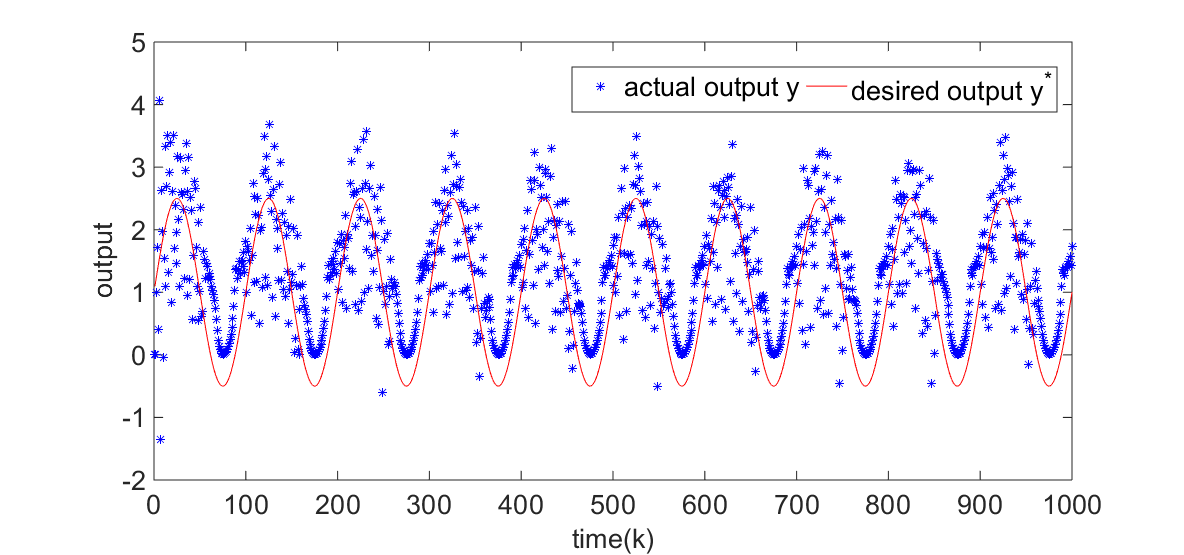
\includegraphics[width=0.65\textwidth ]{ch4-sim-str-y.png}\label{fig.sim.str.y}}\\
	\subfigure[跟踪误差]{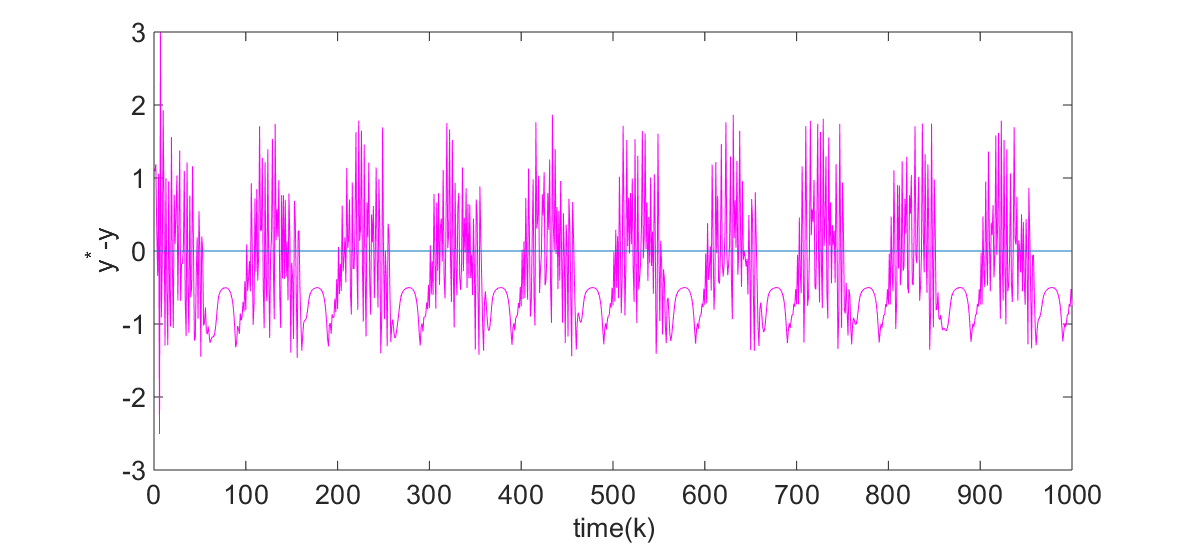
\includegraphics[width=0.65\textwidth ]{ch4-sim-str-yerror.png}\label{fig.sim.str.ye}}
	%\subfigure[控制输入]{\includegraphics[width=0.5\textwidth ]{ch4-sim-elmu.png}\label{fig.sim.elm.u}}
	\caption{系统输出结果:自校正控制算法}
	\label{fig.sim.str.sys}
\end{figure}

造成跟踪控制效果较大差异的重要原因之一,就是两种控制算法中对系统参数估计算法的不同,图\ref{fig.sim.str.sys}展示了仿真得到的参数估计曲线。相对于图\ref{fig.sim.str.theta}中改进的最小二乘算法来说,图\ref{fig.sim.elm.theta}的信息浓缩估计参数估计比较准确。
\begin{figure}[!htb]
	\centering
	\subfigure[信息浓缩估计]{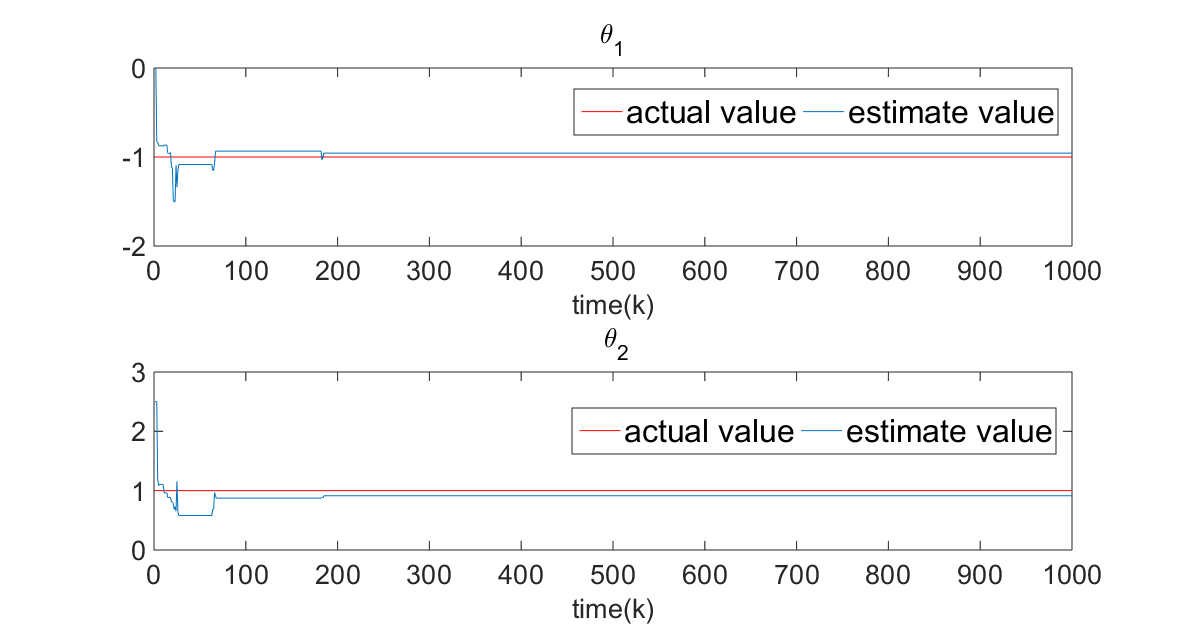
\includegraphics[width=0.65\textwidth ]{ch4-sim-elm-theta.png}\label{fig.sim.elm.theta}}\\
	\subfigure[改进的最小二乘估计]{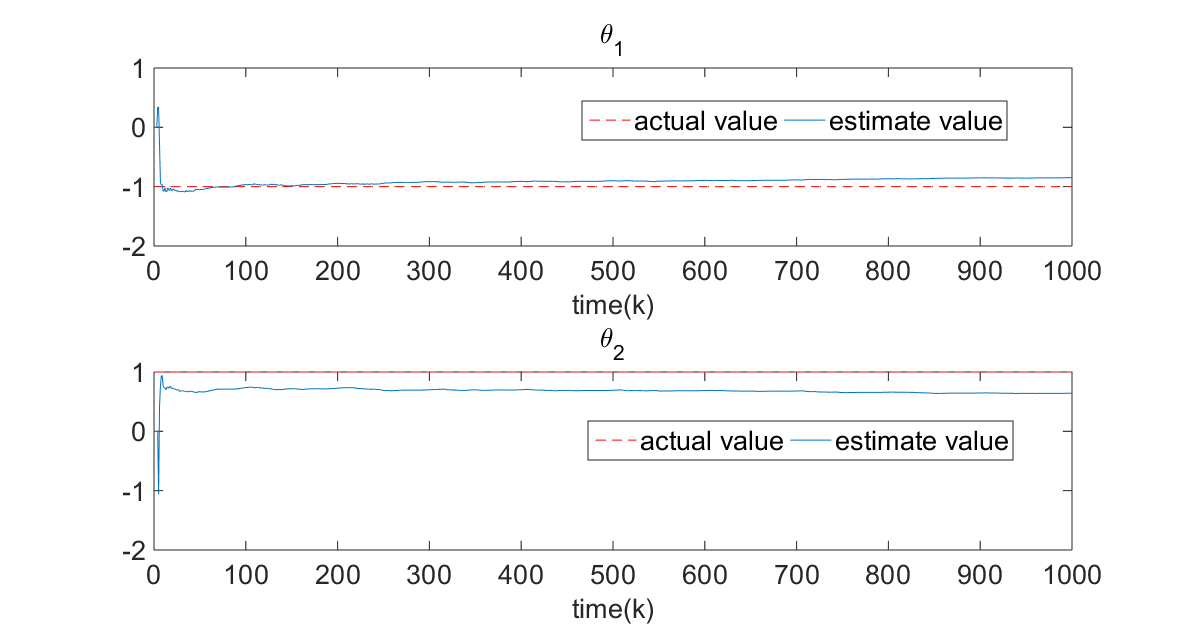
\includegraphics[width=0.65\textwidth ]{ch4-sim-str-theta.png}\label{fig.sim.str.theta}}
	\caption{未知参数估计结果对比}
	\label{fig.sim.str.sys}
\end{figure}

除了对系统参数不确定性的处理外,半参数自适应控制中用在线超限学习机估计非参数部分,估计结果如图\ref{fig.sim.elm.f},选择了径向基函数作为激活函数,网络的隐含层个数在10到20之间。从图中可以,对非线性函数的逼近结果很好,导致对下个周期的非参数部分估计比较准确。这充分说明了引入超限学习机这种机器学习算法大大较少系统的非参数不确定性,从而能够计算出合适的控制输入,给到被控对象。另外,基于超限学习机的网络学习过程也没有影响控制的实时性,计算很快,在普通PC机上(实验计算机配置为Intel i5处理器,主频为2.3GHz)每个周期的估计时间在0.05毫秒以内,如果系统经过裁剪和优化可进一步提高运算速度,基本能够满足基于工业PC的控制系统对实时性的要求。网络学习过程并没有引入一般深度网络依赖的并行计算等复杂设计,有利于在工业嵌入式系统中实现。
\begin{figure}[!htb]
  \centering
  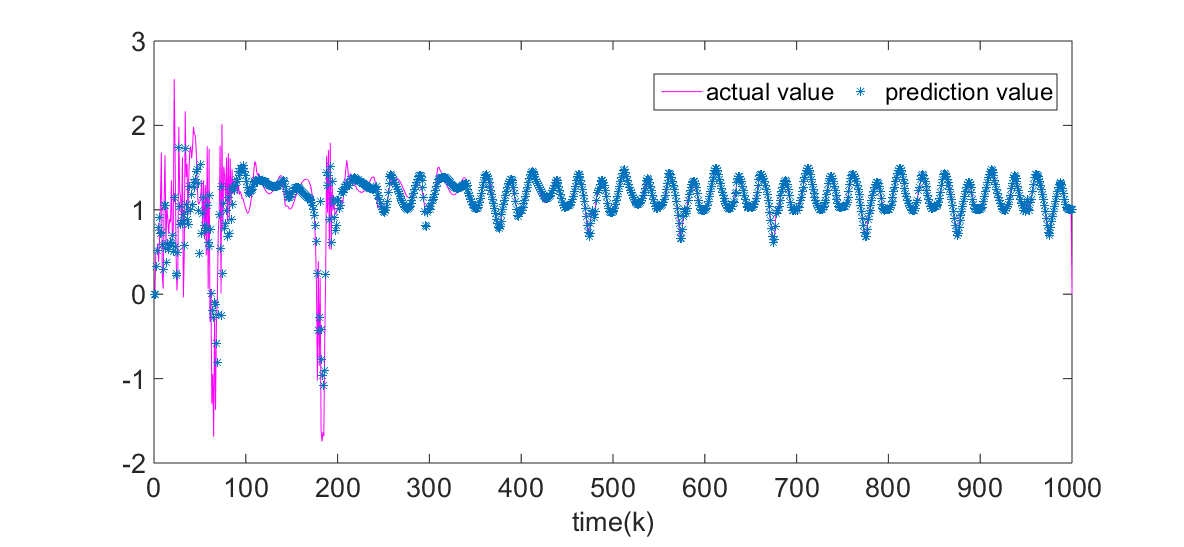
\includegraphics[width=0.7\textwidth ]{ch4-sim-elm-f.png}\\
% e.g.,[scale=0.75], [width=0.75\textwidth ]
  \caption{半参数自适应控制中超限学习机对非参数部分的估计结果}
  \label{fig.sim.elm.f}
\end{figure}

\section{本章总结}\label{sect:4.5}
本章主要设计了基于超限学习机的非线性估计和半参数自适应控制。首先给出了半参数系统的轨迹跟踪问题的数学描述,并分析了半参数模型的自适应估计和控制问题;然后介绍了超限学习机的主要思想、算法特点和改进算法,并用合适的超限学习机变体算法设计了非参数部分的估计算法;接着在信息浓缩和超限学习机的自适应估计基础上,设计了针对半参数系统轨迹跟踪问题的自适应控制器,并分析了闭环跟踪稳定性;最后用仿真实例测试和验证本章设计的半参数自适应控制算法的性能,用改进的自校正控制算法作对比。